\section{Frontend}

\subsection{Tecnologies and libraries}

\subsubsection{ReactJs}
Node.js is an open-source, cross-platform, back-end JavaScript runtime environment that runs on the V8 engine and executes JavaScript code outside a web browser. Node.js lets developers use JavaScript to write command line tools and for server-side scripting—running scripts server-side to produce dynamic web page content before the page is sent to the user's web browser. Consequently, Node.js represents a "JavaScript everywhere" paradigm, unifying web-application development around a single programming language, rather than different languages for server-side and client-side scripts.

\begin{itemize}
    \item \textbf{Used Version:} 17.0.1 
\end{itemize}

\subsubsection{NextJs}
Node.js is an open-source, cross-platform, back-end JavaScript runtime environment that runs on the V8 engine and executes JavaScript code outside a web browser. Node.js lets developers use JavaScript to write command line tools and for server-side scripting—running scripts server-side to produce dynamic web page content before the page is sent to the user's web browser. Consequently, Node.js represents a "JavaScript everywhere" paradigm, unifying web-application development around a single programming language, rather than different languages for server-side and client-side scripts.

\begin{itemize}
    \item \textbf{Used Version:} 10.0.6 
\end{itemize}

\subsubsection{Typescript}
Node.js is an open-source, cross-platform, back-end JavaScript runtime environment that runs on the V8 engine and executes JavaScript code outside a web browser. Node.js lets developers use JavaScript to write command line tools and for server-side scripting—running scripts server-side to produce dynamic web page content before the page is sent to the user's web browser. Consequently, Node.js represents a "JavaScript everywhere" paradigm, unifying web-application development around a single programming language, rather than different languages for server-side and client-side scripts.

\begin{itemize}
    \item \textbf{Used Version:} 4.1.5 
\end{itemize}

\subsubsection{Stripe}
Node.js is an open-source, cross-platform, back-end JavaScript runtime environment that runs on the V8 engine and executes JavaScript code outside a web browser. Node.js lets developers use JavaScript to write command line tools and for server-side scripting—running scripts server-side to produce dynamic web page content before the page is sent to the user's web browser. Consequently, Node.js represents a "JavaScript everywhere" paradigm, unifying web-application development around a single programming language, rather than different languages for server-side and client-side scripts.

\begin{itemize}
    \item \textbf{Used Version:} 8.137.0
\end{itemize}

\subsection{Architectural Overview}

\begin{figure}[H]
    \centering
    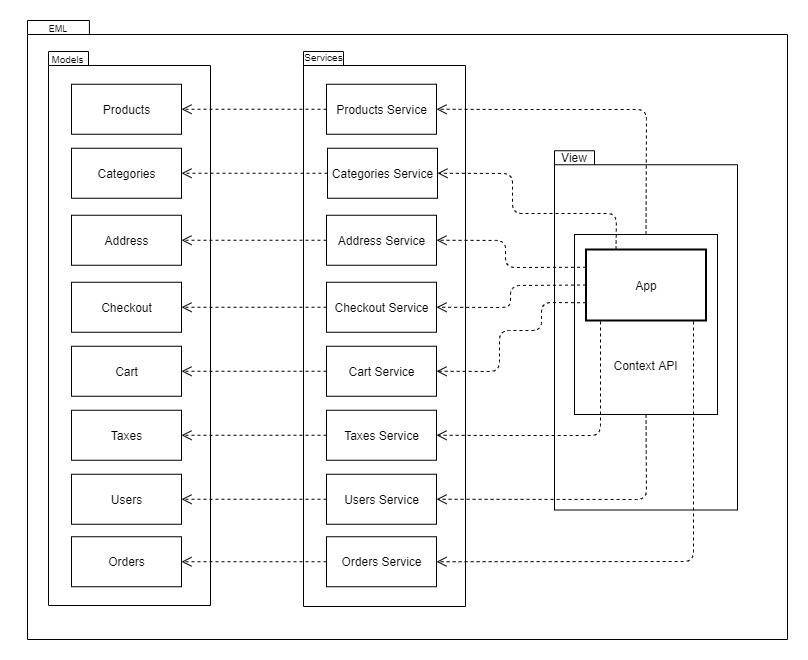
\includegraphics[width=45em]{res/images/\EML-FE.jpg}
\end{figure}

Node.js is an open-source, cross-platform, back-end JavaScript runtime environment that runs on the V8 engine and executes JavaScript code outside a web browser. Node.js lets developers use JavaScript to write command line tools and for server-side scripting—running scripts server-side to produce dynamic web page content before the page is sent to the user's web browser. Consequently, Node.js represents a "JavaScript everywhere" paradigm, unifying web-application development around a single programming language, rather than different languages for server-side and client-side scripts.

\subsubsection{Service's role}

\subsubsection{ContextAPI and the persistence layer}







